\section{Optimization scheme}
\par Again, we clarify the problem setting. We have dataset which is pair of data and label  $\{(\bm{x^{(i)}}, y^{(i)})\}_{i=1,2,\cdots,N}$, where  $y^{(i)}\in\{-1,1\}$. By learning this dataset, we hope to be able to predict suitable labels for unlabeled data. 

\par Assume that we have the following circuit in Figure \ref{fig:abst1}.
\begin{figure}[htb]
    \centering
    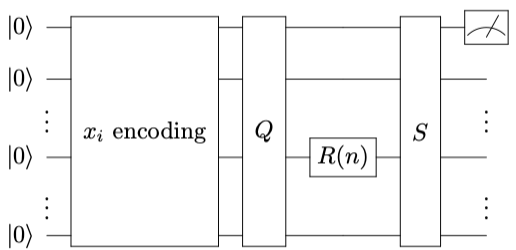
\includegraphics[keepaspectratio, scale=1.5]{method/abst1.png}
    \caption{The fraxis gate that we are interested in and want to optimize is expressed explicitly.}
    \label{fig:abst1}
\end{figure}
Here, $Q$ and $S$ are the unitary operations. Fraxis gate $R(\bm{n})$ is applied to the $d$-th qubit. As seen in Figure \ref{fig:abst1}, the first qubit is measured by observable $Z$ and its value ranges from -1 to 1. This value can be written as following:
$$\upsilon_i=\tr{\left(Z_1 SR_d(\bm{n})Q\rho_{i} Q^\dagger R_d(\bm{n})^{\dagger}S^\dagger\right)}$$
We call this value as $\upsilon_i$ and define it as the prediction value of the label by the quantum circuit in Figure \ref{fig:abst1}. That means:
$$y_i \longleftarrow
\left\{
\begin{array}{ll}
-1 & \ \ \rm{if}\ \upsilon_i<0\\
1 & \ \ \rm{otherwise}\\
\end{array}
\right.
$$

\par Then, we define the cost function like below:
$$-\sum_{i=1}^N y_{i}\upsilon_i$$
Intuitively, when the predicted value and the actual label match, the value of the cost function is reduced, and vice versa.

\par Our method for minimizing the cost function is described below. First, we transform the cost function and see that the cost function can be written in a very simple form. For simplicity of notation, we write $Q\rho_i Q^\dagger$ as $\rho_i$, and $S^\dagger Z_1 S$ as $\mathcal{M}$.
$$
\begin{aligned}
&-\sum_{i=1}^Ny_i\upsilon_i\\
=&-\sum_{i=1}^N y_{i}\tr(\mathcal{M} R(\bm{n}){\rho_{i}}R(\bm{n}^\dagger)\\
=&-\sum_{i=1}^N y_{i} (n_{x}^2\tr(\mathcal{M} X\rho_{i} X)+n_{y}^2\tr(\mathcal{M} Y\rho_{i} Y)+n_{z}^2\tr(\mathcal{M} Z\rho_{i} Z)\\
&+n_{x}n_{y}\tr(\mathcal{M} X\rho_{i} Y+\mathcal{M} Y\rho_{i} X)\\
&+n_{y}n_{z}\tr(\mathcal{M} Y\rho_{i} Z+\mathcal{M} Z\rho_{i}Y)\\
&+n_{z}n_{x}\tr(\mathcal{M} Z\rho_{i} X+\mathcal{M} X\rho_{i} Z))\\
=&-\sum_{i=1}^N y_{i}(n_{x}^2 g_{ix} + n_{y}^2 g_{iy} + n_{z}^2 g_{iz}\\
&+n_{x}n_{y}(2g_{ixy}-g_{ix}-g_{iy})+n_{y}n_{z}(2g_{ixz}-g_{iy}-g_{iz})+n_{z}n_{x}(2g_{iz}-g_{ix}-g_{iz}))\\
=&-\sum_{i=1}^N y_{n}\bm{n}^\top G_{i} \bm{n}\\
=&-\bm{n}^\top\left(\sum_{i=1}^N  y_{n}G_{i}\right)\bm{n}\\
=&-\bm{n}^\top G \bm{n}\\
\end{aligned}
$$
where 
$$
\begin{aligned}
g_{ix}&=\tr(\mathcal{M} X\rho_{i}X)\\
g_{iy}&=\tr(\mathcal{M} Y\rho_{i}Y)\\
g_{iz}&=\tr(\mathcal{M} Z\rho_{i}Z)\\
g_{ixy}&=\tr(\mathcal{M} \frac{X+Y}{\sqrt{2}}\rho_{i}\frac{X+Y}{\sqrt{2}})\\
g_{ixz}&=\tr(\mathcal{M} \frac{X+Z}{\sqrt{2}}\rho_{i}\frac{X+Z}{\sqrt{2}})\\
g_{iyz}&=\tr(\mathcal{M} \frac{Y+Z}{\sqrt{2}}\rho_{i}\frac{Y+Z}{\sqrt{2}})\\
\end{aligned}$$
and
$$G_{i}=
\begin{pmatrix}
g_{ix} & g_{ixy}-\frac{g_{ix}+g_{iy}}{2} & g_{ixz}-\frac{g_{ix}+g_{iz}}{2}\\
g_{ixy}-\frac{g_{ix}+g_{iy}}{2} & g_{iy} & g_{iyz}-\frac{g_{iy}+g_{iz}}{2}\\
g_{ixz}-\frac{g_{ix}+g_{iz}}{2} & g_{iyz}-\frac{g_{iy}+g_{iz}}{2} & g_{iz}\\
\end{pmatrix}
$$
\par All the elements of $G_i$, that means $g_x, g_y, g_z, g_{xy}, g_{xz}, g_{yz}$, is obtained by replacing the fraxis gate $R(\bm{n})$ we focus on now. Therefore, in order to construct the matrix $G$, 6 observations of the quantum circuit are required for every data $\{x_i\}\ (i=1,2,\cdots, N)$.
\par Note, that 
$$G=\sum_{i=1}^N  y_{i}G_{i}$$
is the real symmetric matrix. By the following theorem, the optimal value to minimize the cost function is the maximum eigenvalue of this real symmetric matrix $G$.

\subsubsection{Theorem}
When the matrix $G=\sum_{i=1}^Ny_iG_i$ has eigenvalues $\lambda_1 \leq \lambda_2 \leq \lambda_3$ (corresponding
eigenvectors as $n_1, n_2, n_3$, $\|n_1\|= \|n_2\| = \|n_3\| = 1$), then the followings holds.
$$\argmax_{\|n\|=1} n^\top Gn = n_3$$
$$\max_{\|n\|=1} n^\top Gn = \lambda_3$$
\subsubsection{Proof}
We define the function $f$ and $\hat{\bm{n}}$:
$$f(n,\tau)=n^\top Gn-\tau(\|n\|^2-1)$$
$$\hat{n} = \argmax_{\|n\|=1} n^\top Gn$$

By the method of Lagrange multipliers, at the point $\hat{n}$, there exists 
$\hat{\tau}$ that satisfies the following.
$$\frac{\partial f}{\partial n}(\hat{n}, \hat{\tau} ) = 0$$
By solving these equations, we get
$$2G \hat{n} = \hat{\tau} \hat{n}$$
Here we use the formula $\frac{\partial }{\partial \bm{x}}\bm{x}^\top A\bm{x}=(A+A^\top)\bm{x}$ (see \ref{chap:appendix}).

\par Therefore, $\hat{n}$ is one of the eigenvectors of $G$, $n_1, n_2, n_3$.
Since 
$$\begin{aligned}
n_k^\top Gn_k&=\lambda_kn_k^\top n_k\\
&=\lambda_k\|n_k\|^2_2\\
&=\lambda_k
\end{aligned}$$
holds, from the condtion $\lambda_1\leq\lambda_2\leq\lambda_3$  directory follows $\hat{n}=n_3$.
\\
\\
\\
The discussion so far can be summarized as follows. Assume the quantum circuit to calculate the cost function has one fraxis gate we are now focusing on. We replace this fraxis gate with $X, Y, Z, \frac{X+Y}{\sqrt2}, \frac{X+Z}{\sqrt2}, \frac{Y+Z}{\sqrt2}$, and calculate the value obtained from the replaced quantum circuit for every data. For each data, we construct the matrix $G_i$, and sum up all $G_i$ with the label $y_i$. Finally we get the symmetric matrix $G$, next solve the eigenvector of $G$ which corresponds to the maximum eigenvalue of $G$. This eigenvector is the optimal parameters for the fraxis gate we are focusing now on. The operation of applying the above operations to all the gates included in the quantum circuit is repeated.